\section{Bilder}
\label{sec:bilder}
Normalerweise sind Bilder und Tabellen "`float"' Objekte, das heißt, dass Latex diese Objekte an den bestmöglichen Ort verschiebt. 
\begin{figure}[H]
	\centering
	\includegraphics[height=5cm]{example-image-b} 
	\caption[Dies ist eine kürzere Bildunterschrift (Verzeichnis)]{Dies ist eine längere Bildunterschrift welche unter dem Bild angezeigt wird. Ist keine kurze Unterschrift angegeben so wird diese lange Bildunterschrift im Verzeichnis angezeigt.}
	\label{fig:testbild}
\end{figure}
Will man dies nicht, so kann man mit der Option [H] (hier) das Bild an genau die Stelle im Text platzieren wo man es haben möchte. das bedingt natürlich dass der Platz unter Umständen nicht optimal genutzt wird.
\begin{figure}[H]
	\centering
	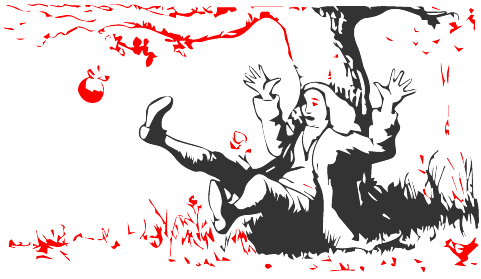
\includegraphics[width=0.7\linewidth]{bilder/newton}
	\caption{Newton entdeckt die Gravitation (sehr abstraktes Bild)}
	\label{fig:newton}
\end{figure}

Mit Latex bzw mit dem Paket TiKz und PGF lässt sich sogar zeichnen. Näheres dazu hier: \href{http://www.texample.net/tikz/examples/}{texample.net}. Es gibt auch die Möglichkeit Graphen und Plots in Latex zu erstellen:
\begin{figure}[H]
	\centering
	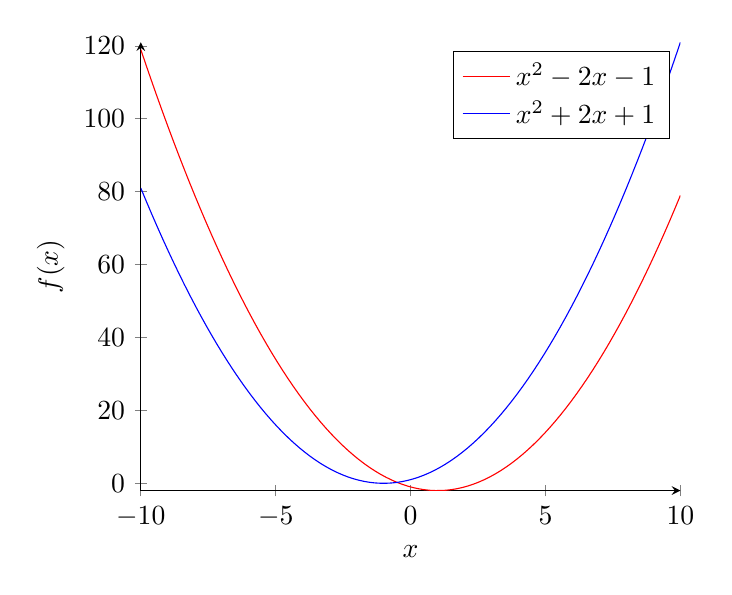
\begin{tikzpicture}
		\begin{axis}[
			axis lines = left,
			xlabel = $x$,
			ylabel = {$f(x)$},
			]
			%Below the red parabola is defined
			\addplot [
			domain=-10:10, 
			samples=100, 
			color=red,
			]
			{x^2 - 2*x - 1};
			\addlegendentry{$x^2 - 2x - 1$}
			%Here the blue parabloa is defined
			\addplot [
			domain=-10:10, 
			samples=100, 
			color=blue,
			]
			{x^2 + 2*x + 1};
			\addlegendentry{$x^2 + 2x + 1$}
		\end{axis}
	\end{tikzpicture}
	\caption{Plot der Funktionen $x^2 - 2x - 1$ und $x^2 + 2x + 1$}
\end{figure}

\begin{figure}[H]
	\centering
\begin{minipage}[c]{0.45\linewidth}
	\begin{tikzpicture}
	\begin{axis}[
	enlargelimits=true,
	legend style
	={
		cells={anchor=east},
		legend pos
		=outer north east,
	},
	]
	\addplot[color=red,only marks,mark size=2.9pt]
	table[x index=0,y index=1] 
	{data/scattered_example.dat};
	\addlegendentry{ds1}
	\addplot[color=blue,only marks,mark=square*,mark size=2.9pt]
	table[x index=0,y index=2] 
	{data/scattered_example.dat};
	\addlegendentry{ds2}
		\addplot[color=green,only marks,mark=triangle*,mark size=2.9pt]
	table[x index=0,y index=3] 
	{data/scattered_example.dat};
	\addlegendentry{ds3}
		\addplot[color=black,only marks,mark=x,mark size=2.9pt]
	table[x index=0,y index=4] 
	{data/scattered_example.dat};
	\addlegendentry{ds4}
	\end{axis}
	\end{tikzpicture}
\end{minipage}
\begin{minipage}[c]{0.45\linewidth}\hspace{1.2cm}
	\begin{tabular}{lllll}
		base&ds1&ds2&ds3&ds4\\ \toprule
		1&5,4&1&1,8&7,2\\
		2&1,8&0,2&8,1&8\\
		3&2,4&0,2&0,9&4,8\\
		4&3,6&1,6&8,1&5,6\\
		5&0,6&1&1,8&6,4\\
		6&4,8&1,4&1,8&2,4\\
		7&5,4&0,2&7,2&3,2\\
		8&6&0,8&0,9&1,6\\
		9&2,4&1&7,2&1,6\\
		10&3,6&0,6&4,5&7,2\\
		11&4,8&1&1,8&3,2\\
		12&3&2&4,5&5,6\\
		13&3&0,4&7,2&5,6\\
		14&4,2&1,8&0,9&8\\
		15&3&2&5,4&5,6
	\end{tabular}
\end{minipage}
\caption{Scatterplot der Datentabelle im bezug zur Basis "`base"'}
\end{figure}
%\begin{figure}[H]
	\centering
	\begin{tikzpicture}[baseline, scale=0.6]
	\pie[rotate=90, /tikz/nodes={text opacity=0,overlay}, color={yellow!40, blue!30}]{2/a, 98/b};
	\end{tikzpicture}
	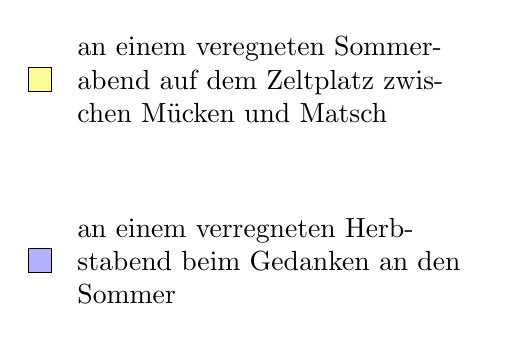
\begin{tikzpicture}[baseline]
	\draw [fill=yellow!40](0,1.0) rectangle (0.3,1.3);
	\node [text width=5cm,align=left, anchor=west] at (0.5,1.15) {an einem veregneten Sommerabend auf dem Zeltplatz zwischen Mücken und Matsch};
	\draw [fill=blue!30](0,-1.0) rectangle (0.3,-1.3);
	\node [text width=5cm,align=left, anchor=west] at (0.5,-1.15) {an einem verregneten Herbstabend beim Gedanken an den Sommer};
	\end{tikzpicture}
	\caption{Wann ein Zelt-Wochenende eine tolle Idee ist}
\end{figure}
\clearpage